
% \xueqing{tick color is green; make the red dash more obvious}  

\section{\detector{} Framework}\label{sec:approach}

To address the two challenges in LLM generation, we employ the following techniques: first, we use supervised fine-tuning and in-context learning to enhance the domain knowledge in LLM; second, we further employ the retrieval-augmented framework (RAG) to enhance the knowledge when SFT is not easy; third, we design a local search technique which alleviates the non-existing package name problem. The \detector{} framework can be found in Figure~\ref{fig: framework} \footnote{Our prompt in Figure~\ref{fig: framework} is: "\emph{Below is a [Programming Language] vulnerability description. Please identify the software name affected by it. Input: [DESCRIPTION]. The top k search results are: [$L_1$][$L_2$]$\cdots$[$L_k$]. Please output the package name in the format "ecosystem:library name".
\#\#\# Response: The affected packages:}". ~\label{fn: input}}.
% \tianyu{using the same input/output format for both fine-tuning and inference}

\subsection{Supervised Fine-Tuning/In-Context Learning}

To solve the first challenge (Section~\ref{sec: empirical_study}), we incorporate supervised fine-tuning~\cite{prottasha2022transfer, church2021emerging} and in-context learning~\cite{dong2022survey, olsson2022context} in \detector{}. For SFT, we use the full training data (Table~\ref{tab: dataset info}); for ICL, we randomly sample 3 examples from the training data for each evaluation vulnerability. For both SFT and ICL, the input and output of the LLM follow the following format: Input: the same prompt as Figure~\ref{fig: framework}~\footref{fn: input}, Output: "\emph{The affected package is [package name]}". The hyper-parameters used for ICL and SFT are listed in Table~\ref{tab: hyper parameter} of Appendix.
% \xueqing{The 3 examples can be seen in Table...of appendix}
% \xueqing{confirm random sampling?} 
% ""\xueqing{fill input}

% \xueqing{For SFT, explain the input/output training data, hyperparameters (appendix), and the fact that we train different models for different PLs }

\subsection{Retrieval-Augmented Generation (RAG)}

%Retrieval augmented generation (RAG) is a framework that enhances the performance of a generative model by injecting the top-k most relevant search result in the prompt~\cite{lewis2020retrieval,gao2023retrieval}. 
To further enhance the LLM's domain knowledge especially when SFT is not easy (e.g., ChatGPT and GPT4), we employ retrieval-augmented generation (RAG) in \detector{}.

\noindent \textbf{Retriever Setting}. Given the description of a vulnerability, our retriever ranks existing package names in an ecosystem (Table~\ref{tab: dataset info}) based on the similarity score between the vulnerability description and the package description. The descriptions of Java, JavaScript, Python, and Go packages are obtained from Maven~\footnote{\url{https://mvnrepository.com}}, NPM~\footnote{\url{https://www.npmjs.com}}, Pypi~\footnote{\url{https://pypi.org}}, and Go~\footnote{\url{https://pkg.go.dev}} documentations.
For example, the description of the package \CodeIn{org.jenkins-ci.plugins:mailcommander} is \textit{``This plug-in provides function that read a mail subject as a CLI Command.''}.
Our retriever follows \cite{vullibminer}'s re-ranking strategy, i.e., first rank all packages (e.g., 435k in Java) using TF-IDF, then re-rank the top 512 packages using a BERT-base model fine-tuned on the same training data in Table~\ref{tab: dataset info}.
% \xueqing{check}

% \xueqing{check consistency with introduction: BERT only vs BERT and TF-IDF}.
% \tianyu{we follow the similar idea of VulLibMiner, use TF-IDF + BERT to retrieve xxx}
% \tianyu{maybe bert-only is ok as the reranking step do not consider TF-IDF}


\subsection{Local Search}

To solve the second challenge (Section~\ref{sec: empirical_study}), we incorporate post-processing in \detector{}.
Based on the empirical study results in Section~\ref{sec: empirical_study}, we design a local search technique to match the generation output with the closest package name from an existing package list (Algorithm~\ref{alg: local search} in Appendix~\ref{sec: local search algorithm}). 

Algorithm~\ref{alg: local search} employs the edit distance as the metric and respects the structure of the package name. Formally, a package name can be divided into two parts: its prefix and suffix (separated by a special character, e.g., `:' in Java).
The prefix (e.g., the artifact ID of Java packages) specifies the maintainer/group of this package, and the suffix (e.g., the group ID of Java packages) specifies the functionalities of this package.
Specifically, Java, Go, and part of JS packages can be explicitly divided while Python and the rest of JS packages only specify their functionalities in their names.
We denote the prefix of a package name as empty if it can not be divided.

Algorithm~\ref{alg: local search} first compares the generated suffix with all existing suffix names and matches the suffix to the closest one. After fixing the suffix, we can then obtain the list of prefixes that co-occur at least once with this suffix. We match the generated prefix with the closest prefix in this list.
The reason that we opt to match the suffix first is twofold. First, our study shows that the vulnerability description more frequently mentions the suffix than the prefix: among all 2,789 vulnerabilities investigated in Section~\ref{sec: empirical_study}, their description mentions 12.4\% of the tokens in the prefixes of the affected packages and 66.0\% of the tokens in their suffixes of the affected packages;
% Specifically, the vulnerability description mentions 12.4\% of the tokens of the prefixes and 66.0\% of the suffixes;
% \tianyu{more explanations}
second, our study also shows that each suffix co-occurs with fewer unique prefixes than conversely.
In all 435k Java packages, each prefix has 5.86 co-occurred suffixes while each suffix has only 1.13 co-occurred prefixes on average.
As a result, it is easier to identify the prefix by first matching the suffix, and then matching the suffix with the co-occurred prefix list. 
% \xueqing{Fix here}
% \xueqing{add study of the frequency to Section 3}
% \xueqing{add study of the frequency to Section 3}

%there exist more suffix package names (e.g., 200k in Java) than prefix package names (e.g., 20k in Java).  
% For example, there are more than 200,000 unique suffixes in the Maven ecosystem and less than 20,000 unique prefixes.
% Therefore, fixing the suffix first reduces LLMs' generation capability less than fixing the prefix first.
% \tianyu{let me consider why}
% \tianyu{correlates to using grammar to reduce syntactical errors, maybe replacing 'local search' with another name}


% Additionally, we conduct a two-staged local search when given a Java vulnerability because the names of Java packages are relatively complex and structural compared to package names of other programming languages. 
% A Java package name consists of its group ID and artifact ID.
% In this scenario, we first search for an existing artifact ID and then search for an existing group ID corresponding to this artifact ID.
% Our rationale is that the artifact IDs include each package's functionalities, which is easier to identify from a vulnerability's description.


% \subsection{During Generation: Constrained Decoding}

% We design our constrained decoding algorithm to restrict the open-source LLMs to include the name of at least one existing package.
% This constraint is written as follows:

% \begin{equation*}
%     \exists l \in \mathcal{L}, \mbox{ s.t. } l \in \mathcal{F}_{generation} (v)
% \end{equation*}

% However, adopting constrained decoding has two technical challenges to address.
% First, each package name contains more than one token (e.g., Python packages have 6 tokens on average) while LLMs generate only one token at once.
% Therefore, we cannot greedily check whether the constraints are satisfied during decoding.
% To address this challenge, we construct a Trie tree to represent the constraints (as shown in Figure~\ref{fig: framework}) and then conduct beam search~\cite{kumar2013beam} to ensure that the output contains at least one path (corresponding to an existing package name) on this Trie tree.

% Second, the large number of packages in each ecosystem (e.g., 435,642 in Maven and 506,848 in Pypi) brings a heavy efficiency burden as the Trie tree for constrained decoding might have more than 1,000,000 nodes. 
% We empirically notice that invoking an LLM with 7B parameters might cost more than 2 hours, which is unacceptable.
% To address this challenge, we relax the ``hard'' constraints to ``soft'' ones.

% Our implementation of ``soft'' constraints consists of two steps.
% (1) We replace the entire Trie tree with a bi-gram Trie tree with only two depth of nodes.
% For example, if a package name consists of three tokens \CodeIn{[``org'', ``google'', ``gson'']}, we add two edges in this bi-gram Trie tree, \CodeIn{``org''} $\rightarrow$ \CodeIn{``google''} and \CodeIn{``google''} $\rightarrow$ \CodeIn{``gson''}.
% The bi-gram Trie tree can remove a large portion (more than 50\%) of leaf nodes in the Trie tree, thus substantially speeding up beam searching during decoding.
% (2) We add another term of probability $\log p_{trie} (w_{i+1}|w_{i})$ to ensure that the output is quite similar to an existing package name.
% Specifically, when decoding the i+1 th token $w_{i+1}$, each token's probability $p(w_{i+1}|w_{0:i})$ is defined as follows:
% \begin{equation*}
%     \begin{aligned}
%         \log p(w_{i+1}|w_{0:i}) \propto &\lambda_{LLM} \log p_{LLM}(w_{i+1}|w_{0:i})\\
%         + &\lambda_{cons} \log p_{trie} (w_{i+1}|w_{i})\\
%         p_{trie}(w_{i+1}|w_{i}) \propto &\ \sum_{l \in \mathcal{L}, j} l[j,j+1] = w[i,i+1]
%     \end{aligned}
% \end{equation*}
% where $\lambda_{LLM}$ and $\lambda_{cons}$ are two hyper-parameters that determine the respective contribution of an LLM and our constraints. 

% \tianyu{is it necessary to mention trie tree with top512 results?}

% % To address this challenge, we follow the similar idea of VulLibMiner, using a TF-IDF~\cite{jones1972statistical, jones2004idf} technique to filter a small candidate of packages.
% % Its empirical results indicate that 512 is a proper candidate size with a recall of at least 0.9.
% % Thus, the decoding constraint is modified as:

% % \begin{equation*}
% % \begin{aligned}
% %     &\mathcal{L}(v) = \mathop{\mbox{Top512}}\limits_{l_i \in \mathcal{L}}\ TF\mathit{-}IDF(v, l_i) \\
% %     &\exists l \in \mathcal{L}(v), \mbox{ s.t. } l \in \mathcal{F}_{generation} (v)
% % \end{aligned}
% % \end{equation*}

% % However, this resolution




% Unlike conventional information retrieval (IR)/classification approaches, \detector{} utilizes the tremendous capabilities of Large Language Models (LLMs) in comprehending vulnerability descriptions.
% Our key insight is that conventional approaches highly depend on their training set and thus face the scalability problem and this problem can be alleviated by modeling this task as a generation task.

% As formalized in Section~\ref{sec: formal}, the training input of \detector{} includes the textual descriptions of vulnerabilities, $\mathcal{V}$, the textual descriptions of all Java libraries in Maven, $\mathcal{L}$, and the mapping relationship from vulnerabilities to libraries, $\mathcal{M}$.
% When applied in practice, \detector{} takes only the textual descriptions of one vulnerability as input and outputs a series of names of libraries affected by this vulnerability.


% \begin{figure}[t]
% \centering
% 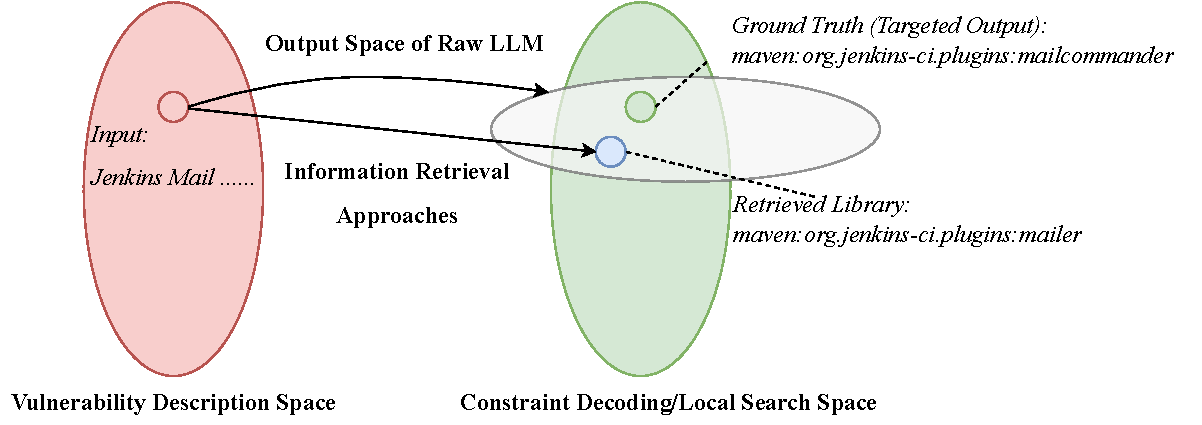
\includegraphics[width=1\linewidth]{figures/approach-illustration.drawio.pdf}
% \caption{An Illustration of the Motivation of our RAG and Constrained Decoding/Local Search Techniques}
% \label{fig: case}
% \end{figure}

% \subsection{Fine-tuning and Prompt-tuning}




% LLMs can correlate the input vulnerability description to vulnerable libraries based on their prior knowledge of these libraries, e.g., their functionalities, usages, and even history issues.

% As formalized in Section~\ref{sec: formal}, the training input of \detector{} includes the textual descriptions of vulnerabilities, $\mathcal{V}$, the textual descriptions of all Java libraries in Maven, $\mathcal{L}$, and the mapping relationship from vulnerabilities to libraries, $\mathcal{M}$.
% When applied in practice, \detector{} takes only the textual descriptions of one vulnerability as input and outputs a series of names of libraries affected by this vulnerability.


% The process of \detector{} is shown in Figure~\ref{fig: framework} with two steps.
% First, we conduct unsupervised fine-tuning on Maven Corpus, which includes all Java libraries and their descriptions.
% This step aims at activating their knowledge of each Java library, including its name and functionalities.
% Second, we conduct supervised fine-tuning on the input dataset $(\mathcal{V}, \mathcal{L}, \mathcal{M})$ to learn the mapping relationship from vulnerabilities to libraries.



% During supervised fine-tuning, we design two specific techniques to improve the effectiveness of \detector{}.
% To help identify zero-shot libraries, we design an input augmentation technique, which feeds the names of vulnerable libraries (a.k.a., recommended libraries) identified by the SOTA approach~\cite{vullibminer} to \detector{} as input.
% This technique provides examples of libraries whose functionalities are likely to be affected by a given vulnerability.
% Thus, \detector{} can generate library names from those with similar functionalities instead of all libraries when \detector{} has no prior knowledge of how these zero-shot libraries are affected by vulnerabilities.
% To address \detector{}'s hallucinations, we design our post-processing technique based on the Levenshtein distance~\cite{levenshtein} to obtain existing Java library names from the response of LLMs.
% We find that \detector{} can generate the components of the targeted library names (i.e., the targeted functionalities and scopes), and make mistakes when jointing these components of library names, thus leading to hallucinations.
% Therefore, hallucination library names are close to the targeted names of vulnerable libraries, and their closest library names tend to be the targeted names.


% \subsection{Two Stages of Fine-Tuning with Input Augmentation}
% \detector{} mainly consists of two stages of fine-tuning on LLMs.
% In this paper, we choose one of the state-of-the-art (SOTA) open-source LLMs, LLaMa~\cite{llama}, as our base LLM with 7B and 13B parameters.

% During unsupervised fine-tuning, \detector{} takes the input of one library description, and its targeted output is its library name.
% Table~\ref{tab: lib-aws} shows an example case in this step.
% Its input describes the functionality of this package, e.g., configuration on AWS plugins, and its output is a structural Java library name, \CodeIn{maven:io.jenkins.plugins: aws-global-configuration}.
% The rationale of unsupervised fine-tuning is to activate their knowledge of each Java library by correlating each Java library's functionality description with its name. 

% After unsupervised fine-tuning, \detector{} conducts supervised fine-tuning on the input dataset, $(\mathcal{V}, \mathcal{L}, \mathcal{M})$ with two steps.
% First, \detector{} invokes another approach of identifying vulnerable libraries to recommend a list of vulnerable library names for input augmentation.
% Note that our rationale for input augmentation is to help identify zero-shot libraries because LLMs have no prior knowledge of how these libraries are affected, so we choose two representative approaches that effectively identify zero-shot libraries.
% Specifically, we choose VulLibMiner and the TF-IDF matcher in VulLibMiner because each of them identifies zero-shot and full-shot (non-zero-shot) libraries with a similar F1 score~\cite{vullibminer} while the TF-IDF matcher, as a NER approach, is less effective than VulLibMiner.
% Second, \detector{} concatenates the description of a given vulnerability with the recommended libraries as the input prompt used for supervised fine-tuning.
% The targeted output in this step is a name list of vulnerable libraries that are affected by this vulnerability.

% Table~\ref{tab: cve-mail} shows an example case of \CodeIn{CVE-2020-2318} in this step.
% The description of this vulnerability mentions the vulnerable functionality, \CodeIn{Jenkins Mail Commander Plugin}, its package source, \CodeIn{Jenkins-ci Plugin 1.0.0}, and how this vulnerability is exploited.
% We also show that the recommended library is another Java library with the same group id and a similar artifact id.
% However, \detector{} rejects this recommended result and outputs the correct vulnerable library, thus indicating its generation capability instead of simply judging whether recommended libraries are correct or not.







% \subsection{Post-Processing of Library Names}





% \begin{algorithm}[t]
% \caption{Post-Processing of Library Names}
% \label{alg: post-processing}
% \begin{algorithmic}[1]
% \Require $rawResponse$, raw text of LLM's Response.
% \Require $libMaven$, Java library names from Maven.
% \Ensure $vulnNames$, a list of vulnerable library names.
% \Function{Post-Processing}{$rawResponse, libMaven$}
%     \State $rawNames \gets rawResponse.findall(\mbox{``maven:\textbackslash 
%  w*:\textbackslash w*''})$
%     \State $artifacts \gets \emptyset{}, groups \gets \{ \}$
%     \For{$mavenName \in libMaven$}
%         \State $\mbox{``maven''}, groupid, artifactid \gets mavenName.split()$
%         \State $artifacts.append(artifactid)$
%         \State $groups[artifactid].append(groupid)$
%     \EndFor
%     \For{$rawName \in rawNames$}
%         \State $\mbox{``maven''}, groupid, artifactid \gets rawName.split()$
%         \State $Levenshtein.weight \gets (W_{insert}, W_{delete}, W_{replace})$
%         \State $artifactid^{\prime} \gets \mathop{argmin}\limits_{id \in artifacts}{Levenshtein(artifactid, id)}$
%         \State $subgroups \gets groups[artifactid^{\prime}]$
%         \State $groupid^{\prime} \gets \mathop{argmin}\limits_{id \in subgroups}{Levenshtein(groupid, id)}$
%         \State $vulnNames \gets \mbox{``maven''}: groupid^{\prime}: artifactid^{\prime}$
%     \EndFor
%     \State \Return{$vulnNames$}
% \EndFunction
% \end{algorithmic}
% \end{algorithm}

% To address \detector{}'s hallucinations, we design our post-processing technique based on the Levenshtein distance~\cite{levenshtein} to obtain existing Java library names from the response of LLMs.
% We find that \detector{} can generate the components of the targeted library names (i.e., the targeted functionalities and scopes), and make mistakes when jointing these components of library names, thus leading to hallucinations.
% Therefore, hallucination library names are close to the targeted names of vulnerable libraries, and their closest library names tend to be the targeted names.



% To address \detector{}'s hallucinations, we design our post-processing algorithm based on the Levenshtein distance~\cite{levenshtein} to obtain correct Java library names from the response of LLMs.
% Our goal is to ensure that the generated library names belong to existing Java libraries.
% One major difficulty for this problem is that Java library names are relatively complex and structural when compared with library names of other programming languages.
% A correct Java library name consists of its group id and artifact id.
% Here we take only libraries collected in Maven into consideration, so we add a prefix identifier, \CodeIn{maven}, before each library name.
% Thus, an example of correct Java library names is \CodeIn{maven:com.google.code.gson:gson}.

% Our post-processing algorithm is designed based on the rationale that hallucinations library names are slightly different from the real names of vulnerable libraries.
% For example, the group id of a Java library consists of multiple components separated by periods (\CodeIn{.}) and some of these components might be neglected or incorrectly replaced.
% Therefore, we use Levenshtein distance to find the correct affected libraries.

% Our technique is shown in Algorithm~\ref{alg: post-processing}.
% It takes the raw-text output of our fine-tuned LLM and outputs a list of vulnerable library names after post-processing.
% This algorithm conducts post-processing through two steps: parsing the raw-text output into a list of library names, and identifying their closest existing library names.

% In Line 2, we parse the raw-text output into a list of library names.
% Here we use a regex expression that contains the identifier ``maven'', group id, and artifact id, to extract library names from our fine-tuned LLM's output, $rawResponse$.

% In Lines 3-16, we identify the closest library names based on the library names extracted in the first step.
% In Lines 3-8, we divide the names of all Java libraries in Maven into multiple groups where library names in each group have the same artifact id.
% In Lines 9-10, for each generated library name, we first split it into its group id and artifact id.
% In Line 12, we use its artifact id, $artifactid$ to find its closest and existing artifact id, $artifactid^{\prime}$.
% Then in Lines 13-14, we use its group id, $groupid$ to find its closest and existing group id, $groupid^{\prime}$ from library names with the same artifact id, $artifactid^{\prime}$.
% Then, we concatenate the ``maven'' identifier with the search results, $groupid^{\prime}$ and $artifactid^{\prime}$ as one post-processed library name.
% Additionally, in Line 11, we manually set the weight used in calculating Levenshtein distances because LLMs change the library names in terms of tokens instead of characters.
% Thus, the weight of inserting one character should be smaller than that of deleting and replacing one, and we set the empirical Levenshtein weights as follows, $W_{insert} = 1, W_{delete} = 4, W_{replace} = 4$.
% \begin{equation}
%     W_{insert} = 1, W_{delete} = 4, W_{replace} = 4
% \end{equation}

% Our empirical statistics show that the average length of tokens in library names is 5.7, and their average number of different characters is 1.7



% \tianyu{group id reflect the sources of library, artifact id reflects its functionalities}

% \CodeIn{maven:com.sdklite:gson}
% Thus, library names generated by LLMs might neglect part of the components or include more components.


% \begin{table}[t]
% \renewcommand\arraystretch{1}
% \centering
% \caption{An Example of Java Library}
% \label{tab: lib-aws}
% \begin{tabular}{p{1.8cm}|p{6cm}}
% \toprule
% Input Prompt              & Below is a Java lib description \\
% \midrule
% \makecell[l]{Library\\ Description} & \makecell[l]{Input: Configure all AWS related plugins from\\ a single page.} \\
% \midrule
% \makecell[l]{Model\\ Response} & \makecell[l]{This package's name is\\ \textit{maven:io.jenkins.plugins:aws-global-configuration}.}\\
% \bottomrule
% \end{tabular}
% \end{table}


% \begin{table}[t]
% \centering
% \caption{An Example of CVE-2020-2318}
% \label{tab: cve-mail}
% \begin{tabular}{p{1.8cm}|p{6cm}}
% \toprule
% Input Prompt              & Below is a Java vulnerability description.   Please identify the software name affected by it \\
% \midrule
% Vulnerability Description & Input: Jenkins Mail Commander Plugin for Jenkins-ci Plugin 1.0.0 and   earlier stores passwords unencrypted in job config.xml files on the Jenkins   controller where they can be viewed by users with Extended Read permission,   or access to the Jenkins controller file system. \\
% \midrule
% \makecell[l]{Recommended\\ Library}       & \makecell[l]{Top 1 search result are \textit{maven:org.jenkins-ci.plugins:job-direct-mail}} \\
% \midrule
% \makecell[l]{Model\\ Response} & \makecell[l]{The affected packages is\\ \textit{maven:org.jenkins-ci.plugins:mail-commander.}}\\
% \midrule
% \makecell[l]{Post-processed\\ Library}    & \makecell[l]{\textit{maven:org.jenkins-ci.plugins:mailcommander}} \\
% \bottomrule
% \end{tabular}
% \end{table}